\documentclass[12pt,oneside]{book}
\usepackage[letterpaper, left=1.2in, right=1in, top=1in, bottom=1in]{geometry}
\usepackage{fancyhdr}
%\pagestyle{fancy}		% add Heading of Chapter on top of each page
\pagestyle{plain}
\fancyhf{}
\rhead{\thepage}
\lhead{\leftmark}
\renewcommand{\chaptermark}[1]{\markboth{\MakeUppercase{#1}}{}}
% \pagestyle{headings}
\usepackage{titlesec}
\usepackage{titletoc}
\usepackage{lipsum}
% \usepackage{fmtcount} % for textual representation of numbers
\titleformat{\chapter}[display]{\normalfont\huge\bfseries}{\chaptertitlename\thechapter}{0pt}{\Huge}
\usepackage{enumitem}
\usepackage{makecell}
\usepackage{adjustbox}
\usepackage{float}
\usepackage{amsmath,amssymb,amsthm,amsfonts}
\usepackage{soul}
\usepackage{frcursive}
\usepackage{algorithmic}
\usepackage{graphicx}
\usepackage{subcaption}
\usepackage{booktabs, multirow} % for borders and merged ranges
\usepackage{tocloft}
% \renewcommand{\chaptername}{}
% \renewcommand{\thechapter}{}
\renewcommand{\cftchapfont}{\bfseries}
\renewcommand{\cftchappagefont}{\bfseries}
% \renewcommand{\cftchappresnum}{Chapter }
% \renewcommand{\cftchapaftersnum}{:}
% \renewcommand\cftchapafterpnum{\vskip 1pt}
% \renewcommand{\cftchapnumwidth}{1em}

\renewcommand*\cftfigpresnum{Figure~}
\settowidth{\cftfignumwidth}{\cftfigpresnum}
\renewcommand{\cftfigaftersnumb}{\quad~}
\setlength{\cftfignumwidth}{4em}

\renewcommand*{\cfttabpresnum}{Table~}
\settowidth{\cfttabnumwidth}{\cfttabpresnum}
\renewcommand{\cfttabaftersnumb}{\quad~}
\setlength{\cfttabnumwidth}{4em}

\usepackage[nottoc,notlof,notlot]{tocbibind}
\usepackage{soul}% for underlines
\usepackage[table]{xcolor} % for cell colors
% \usepackage{} % Change to other font if needed
\usepackage{setspace}
% \usepackage{textcomp}
\usepackage{xcolor}
\usepackage[bookmarks=true, hidelinks]{hyperref}

\usepackage[utf8]{inputenc}

\usepackage[backend=biber,style=ieee,sorting=none]{biblatex} % ieee citaion style
%\usepackage[backend=biber,style=apa]{biblatex} % apa citation style

\usepackage{hyphenat}

\usepackage{appendix}
\usepackage{listings}
\usepackage{bm}
% \usepackage{natbib}
\setcounter{tocdepth}{2}
\setcounter{secnumdepth}{5}
\bibliography{Reference}
\addbibresource{Main.bib}
\usepackage{titlesec}
% \titlespacing*{\chapter}{0pt}{0pt}{30pt}
% \titleformat{\chapter}[display]{\normalfont\huge\bfseries\centering}{\centering\chaptertitlename\ \thechapter}{0pt}{\Huge}
\titlespacing*{\chapter}{0pt}{0pt}{30pt}
\titleformat{\chapter}[display]{\normalfont\huge\bfseries\centering}{}{-90pt}{\Huge}

% table row color macro
\usepackage[first=0,last=9]{lcg}
\newcommand{\ra}{\rand0.\arabic{rand}}

\begin{document}
\doublespacing

%%%%%%%%%%%%%%%%%%%%%%%%%%%%%%%%%%%%%%%%%%
%% Additional Material
%%%%%%%%%%%%%%%%%%%%%%%%%%%%%%%%%%%%%%%%%%

% Title Page
%========================================
%% Define your thesis title, your name, your department, your degree, and your month and year of graduation here

\newcommand{\thesisTitle}{PrintShop: Assessing OS and Capabilities of Serial Print Devices}
\newcommand{\yourName}{Micah Flack}
\newcommand{\yourDept}{Beacom College of Computer and Cyber Sciences}
\newcommand{\yourDegree}{Doctor of Philosophy}
\newcommand{\yourMajor}{Cyber Operations}
\newcommand{\yourMonth}{September 21,}
\newcommand{\yourYear}{2023}
%%%\newcommand{\yourCommitteeChair}{Dissertation chair}
%%%\newcommand{\yourCommitteeMemberA}{Dr. Someone Name}
%%%\newcommand{\yourCommitteeMemberB}{Dr. Another Person}
%%%\newcommand{\yourCommitteeMemberC}{...}


%%%%%%%%%%%%%%%%%%%%%%%%%%%%%%%%%%%%%%%%%%%%%%%%%%%%%%%%%
% Do not edit these lines unless you wish to customize the template
%%%%%%%%%%%%%%%%%%%%%%%%%%%%%%%%%%%%%%%%%%%%%%%%%%%%%%%%%

\begin{titlepage}
\begin{center}

\begin{center}
    
\includegraphics[width=0.3\columnwidth, keepaspectratio]{Additional/DSULogo.png}\\
\end{center}

\vspace*{0.5in}

\begin{doublespacing}

{\LARGE{\MakeUppercase{\thesisTitle}}}\\
\vspace{\baselineskip}
\vfill
Research Proposal\\
\vspace{\baselineskip}
\yourDegree\\
in\\
\yourMajor\\
\vspace{\baselineskip}
\yourMonth{} \yourYear{}\\
\vspace{\baselineskip}
By\\
\vspace{\baselineskip}
\yourName\\
\vspace{\baselineskip}
%%%Dissertation Committee:\\
%%%\yourCommitteeChair\\
%%%\yourCommitteeMemberA\\
%%%\yourCommitteeMemberB\\
%%%\yourCommitteeMemberC\\
\vspace{\baselineskip}
\yourDept \\

\end{doublespacing}

\end{center}
\end{titlepage}
\currentpdfbookmark{Title Page}{TitlePage}

\pagenumbering{roman}
\setcounter{page}{2}

% Dissertation Approval Form
%=========================================
% \input{Additional/ApprovalForm}
% \clearpage


% Acknowledgements
%=========================================
% \input{Additional/Acknowledgements}
% \clearpage

% Abstract
%=========================================
% \begin{abstract}
(OUTLINE FILLER WORDS) pharetra sit amet aliquam id diam maecenas ultricies mi eget mauris pharetra et ultrices neque ornare aenean euismod elementum nisi quis eleifend quam adipiscing vitae proin sagittis nisl rhoncus mattis rhoncus urna neque viverra justo nec ultrices dui sapien eget mi proin sed libero enim sed faucibus turpis in eu mi bibendum neque egestas congue quisque egestas diam in arcu cursus euismod quis viverra nibh cras pulvinar mattis nunc sed blandit libero volutpat sed cras ornare arcu dui vivamus arcu felis bibendum ut tristique et egestas quis ipsum suspendisse ultrices gravida dictum fusce ut placerat orci nulla pellentesque dignissim enim.
(OUTLINE FILLER WORDS).
\end{abstract}

\begin{IEEEkeywords}
serial devices, thermal printer, PoS, ICS, badusb, hardware hacking, embedded devices. 
\end{IEEEkeywords}
% \clearpage

% Declaration 
%=========================================
% \input{Additional/Declaration.tex}
% \clearpageContents

% \begin{singlespace}
%     \setlength\cftbeforefigskip{\baselineskip}
%     \Abstract
% \end{singlespace}
% \setcounter{page}{3}

% Acknowledgements Page (optional)
%========================================
%\pagenumbering{roman} % Uncomment if Copyright page is not in use
% \addcontentsline{toc}{chapter}{Acknowledgments}
% %\setcounter{page}{2} % Uncomment if Copyright page is not in use
% \input{Additional/Acknowledgements.tex}


% Table of Contents
%========================================
% \pagenumbering{roman} % Uncomment if Copyright and Acknowledgements are not in use
% \setcounter{page}{2} % Uncomment if Copyright and Acknowledgements are not in use

% \renewcommand{\cftchapdotsep}{\cftdotsep}
\renewcommand{\contentsname}{\hfill \Large \uppercase{Table of Contents}\hfill}   
\renewcommand{\cftaftertoctitle}{\hfill}
\addcontentsline{toc}{chapter}{Table of Contents}
% \begin{doublespacing}
\tableofcontents
\clearpage
% \end{doublespacing}
% \currentpdfbookmark{Table of Contents}{TOC}


%%% UNCOMMENT FOR FINAL PUB

% %%% Uncomment triple comments for List of Tables
% % List of figures and tables
% %========================================
% % \addcontentsline{toc}{chapter}{List of Tables}
% \renewcommand{\listtablename}{\hfill \Large \uppercase{List of Tables} \hfill}
% \addcontentsline{toc}{chapter}{List of Tables}
% % \begin{singlespace}
% % 	\setlength\cftbeforetabskip{\baselineskip}
% \listoftables
% % \end{singlespace}
% \clearpage

% %%% Uncomment triple comments for List of Figures
% % \addcontentsline{toc}{chapter}{List of Figures}
% \renewcommand{\listfigurename}{\hfill \Large \uppercase{List of Figures} \hfill}
% \addcontentsline{toc}{chapter}{List of Figures}
% % \begin{siwnglespace}
%     % \setlength\cftbeforefigskip{\baselineskip}
% \listoffigures
% % \end{singwlespace}
% \clearpage


%%%%%%%%%%%%%%%%%%%%%%%%%%%%%%%%%%%%%%%%%%
%% Main Content
%%%%%%%%%%%%%%%%%%%%%%%%%%%%%%%%%%%%%%%%%%

% resume page numbering for rest of document
\pagenumbering{arabic}
\setcounter{page}{1} % set the page number appropriately

% Chapter 1
\chapter{\leavevmode Introduction}
\label{chap:introduction}

% \section*{Overview}
% \addcontentsline{toc}{section}{Overview}
\section{Background}  \label{background}

Serial printers are devices commonly used for instant reporting of system data for industrial control systems (ICS) and receipts for point-of-sale (POS) systems. These devices are connected to their host using Wi-Fi, bluetooth, ethernet, or USB; in some cases, serial RS232 is an option as well. The goal of this research is to assess what software and hardware protections are enabled, as well as, how configurable the serial printers are for further exploit research.


\begin{figure}[ht]%
  \centering
  \subfloat[\centering Square POS]{{ 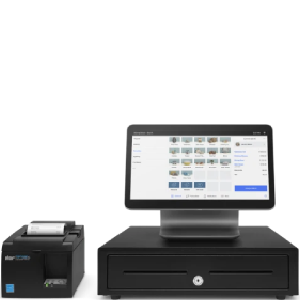
\includegraphics[width=0.30\textwidth,keepaspectratio]{Figures/MidSquare.png} }}%
  \qquad
  \subfloat[\centering SurePOS]{{ 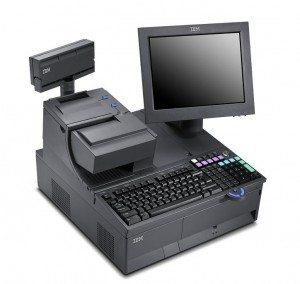
\includegraphics[width=0.25\textwidth,keepaspectratio]{Figures/SurePOS.jpg} }}%
  \caption{Comparison of common POS systems}%
  \label{fig:comparison_pos}%
\end{figure}

Figure \ref{fig:comparison_pos} shows us two similar looking point-of-sale systems. However, the operating system and required hardware used by both is different. Typically, unless you have the Square provided terminal, their software/client is installed onto an Android or iOS device and connected to a Square compatible card reader \autocite{ondrusMobilePaymentsMarket2011}. Whereas, the SurePoS, NCR, or other common EFTPoS system will run a proprietary OS based on Windows or Linux \autocite{ebimoboweiROLESOFTWARECASHLESS2018}. Furthermore, these PoS require some form of printing receipts as record keeping for the business owner and customer. And these devices also vary in terms of processing capabilities and operating system.

For instance, a common thermal printer seen with PoS systems, integrated with fuel pumps, or other industrial control equipment, is the SNBC BTP-S80 thermal printer \autocite{SNBCBTPS80Thermala,SNBCNewBeiyangIntelligent}. There are multiple versions of the device with support for Bluetooth, USB only, or combination of USB/Serial/Ethernet. The bluetooth hardware is provided over an accessory 25-pin serial connection, with more I/O as a serial connection via RS232C connector and USB Type-B. It has driver support for various platforms: Android, iOS, Windows, Linux, and MacOS. The most interesting aspects are the processor, an Arm Cortex M4 clocked at 3.54MHz, and the operating system, a proprietary version of FreeRTOS. The system architecture is Armv7E-M with JTAG/SWD hardware debugging support \autocite{CortexM4,FreeRTOSMarketLeading}.

By default, the printer has enough headroom to process ESC/POS commands for printing paper and a webserver for debugging or general diagnostics. In theory, the uncompromised device could be flashed with modified firmware to act as a decoy and human-input-device (HID) against the host PoS. The viability of any vulnerabilities would likely be dependent upon supply chain attacks or physical bait-and-switch tactics \autocite{scaifeFearReaperCharacterization2018}.

% In this paper, we propose exploring the processing capabilities and extensibility of FreeRTOS to act as a dual HID clone and printer for continued research.

\section{Significance}  \label{significance}

According to the Federal Trade Commission (FTC), there were 37,932 reports of credit card fraud in 2012 and 87,451 reports in 2022 \autocite{ConsumerSentinelNetwork2023,forthesentinelConsumerSentinelNetwork2022}. This marks an increase of credit card payment fraud by an estimated, 30.5\%. By comparison, since 2020, there has been a 14.6\% increase in credit card related fraud. Which does not include the millions of other fraud reports the FTC receives every year. In 2022 alone, there were around 5.1 million fraud, identity theft, and miscellaneous reports in total \autocite{ConsumerSentinelNetwork2023,forthesentinelConsumerSentinelNetwork2022}. The statistics for these reports stresses how crucial the security of payment systems are, both physical and online. And, the need to secure them grows every year.

Spyduino is \autocite{karystinosSpyduinoArduinoHID2019} a working example of a programmable BadUSB device using an Arduino to mimic a Human Interface Device (HID). Arduinos are typically more accessible and easily developed compared to an embedded device whose design is more single purpose \autocite{griffithsECIAIR2019European2019,patnaikpatnaikuniComparativeStudyArduino2017}. Especially if the goal is to not modify hardware or require hands-on access for exploitation. However, the research shows us that is it possible create HID clones from scratch if the hardware is compatible.

The Arduino used in their research is powered by an ATmega328P microcontroller with 32KB flash memory, 2KB SRAM, and 1KB EEPROM. Compared to the most likely target device of our proposed research, the SNBC BTP-S80, it features an ARM Cortex M4 microcontroller with 512KB flash memory, 96KB SRAM, 4KB of EEPROM. This is relevant to the proposed research, because it shows that a device with similar hardware specifications was feasible; meaning, it is likely that our own research will be successful. BadUSBs are a known and tested area of research. The novelty of this proposal comes from the assessment of the printer devices and showing whether one could be used maliciously within their environments (e.g., PoS systems, or ICS).

\section{Research Goals and Objectives}  \label{researchgoalsobjectives}

This research primarily focuses on physical POS systems or terminals and their hardware (serial accessories), rather than online solutions. For instance, not mobile payment apps like Venmo, CashApp, Zelle, or Paypal \autocite{wangMobilePaymentSecurity2016} since their environments typically do not use serial print devices. It is also likely that more research would be needed for emulating touch inputs for mobile environments versus the traditional keyboard attacks that will be implemented. Presumably, the host-to-guest communication will not differ greatly
between other environments (e.g., ICS). If the printers have demonstrable weaknesses with an Ubuntu host, that will fulfill the testing requirements.

The goal of this research is to further establish academic works in regards to embedded printer devices testing and security. This area is loosely documented within academia and only mentioned vaguely in relation to statistical reports or applied research using entirely different environments. For instance, most researchers limit their analysis of the environment to smartphones and the corresponding payment app, or detection systems for card skimmers \autocite{scaifeFearReaperCharacterization2018}.

Through this research we hope to identify supply chain risks using side channel attacks from auxiliary devices. Some examples of how the research could be applied in the future vary: BadUSB/BashBunny \autocite{hak5BashBunny}, JuiceShop \autocite{OWASPJuiceShop}, DVWA \autocite{woodDAMNVULNERABLEWEB2023}, or Webgoat \autocite{OWASPWebGoatOWASP}. Works within the PoS system context or embedded systems discussing supply chain attacks through third-party hardware are limited.

% \section{Printers}  \label{printers}

% \begin{figure}[ht]%
%   \centering
%   \subfloat[\centering BTP-S80]{{ 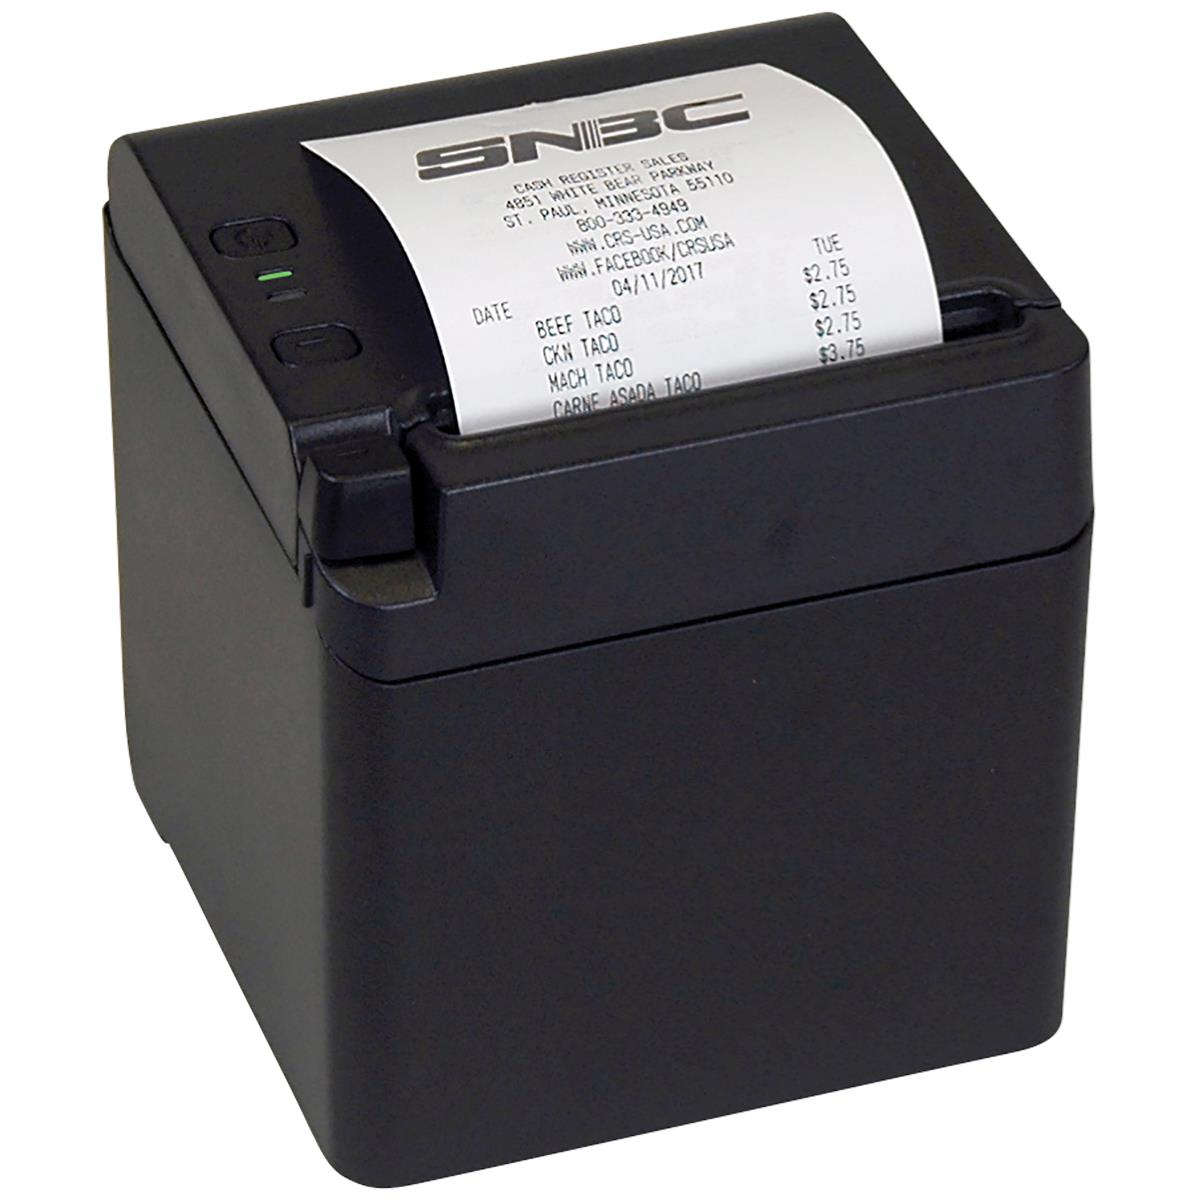
\includegraphics[width=0.40\textwidth,keepaspectratio]{Figures/SNBC_S80.jpeg} }}%
%   \qquad
%   \subfloat[\centering Printer I/O]{{ 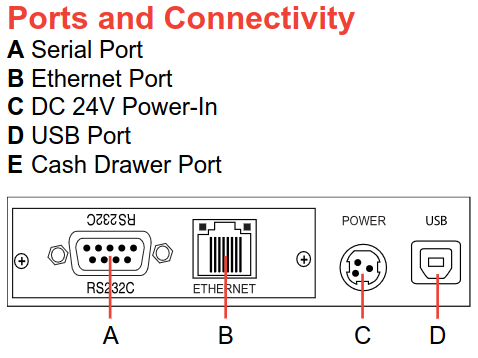
\includegraphics[width=0.40\textwidth,keepaspectratio]{Figures/SNBC_S80_IO.png} }}%
%   \caption{SNBC BTP-S80}%
%   \label{fig:btp_s80}%
% \end{figure}

% Figure \ref{fig:comparison_pos} shows us two similar looking point-of-sale systems, albeit one is much older looking. However, the operating system and required hardware is very different. Typically, unless you have the Square provided terminal, their software/client is installed onto an Android or iOS device and connected to a Square compatible card reader \autocite{ondrusMobilePaymentsMarket2011}. Whereas, the SurePoS, NCR, or other common EFTPoS system will run a proprietary OS derived from Windows or Linux \autocite{ebimoboweiROLESOFTWARECASHLESS2018}. Furthermore, these PoS tend to require some form of printing receipts as record keeping for the business owner and customer. And these devices also vary in terms of processing capabilities and operating system.

\section{Research Questions}  \label{researchquestions}

The research questions that this proposal seeks to answer are as follows:
\begin{itemize}
  \item Q1: Can the hardware be reflashed with a modified firmware image (e.g., FreeRTOS, ReconOS, VxWorks)? Testing a version of the original firmware with additional libraries, or an alternative OS, allows us to see if supply chain attacks are a concern. Either by the manufacturer, supplier, or other party. Reflashing is not novel by itself, however, the device might have protections in place to prevent it.  
  \item Q2: Does the hardware and firmware have enough resources to support HID functionality on-top of printing? In other words, can we maintain operation of standard printer command interpretation and side-channel input attacks without causing crashes or delays? The viability of the attack depends on it going unnoticed by operators or technicians. 
  \item Q3: Besides HID cloning, what other threat areas are exposed (e.g., network stack, web management portal, memory protections)? Are there any identifiable or known exploits when accessing the configuration panel (e.g., HTTP/2)? These provide a non-invasive method for bootstrapping the device.
\end{itemize}

Each of these goals will be approached individually as prescribed by the methodology.

% Uncomment chapters as they are completed...

% % Chapter 2
% \section{Related Works}

\subsection{RTOS: Software and Security}
\autocite{Benadjila2018WooKeyU} introduces several embedded kernels and discusses their differences regarding developing a secure mass storage device. For this research, we are primarily interested in RTOS-like kernels because of existing support for a sample device like the SNBC BTP-S80 printer. However, the paper criticizes such operating systems because their "real-time driven design is largely incompatible with the overhead produced by security mechanisms." For many applications, there is a trade-off with RTOS where performance is the main criterion and security is not a priority. \autocite{yuRealTimeOperatingSystem} introduces several common RTOS and discusses their security issues. Notably, most RTOS are susceptible to code injection, cryptography inefficiency, unprotected shared memory, priority inversion, denial of service attacks, privilege escalation, and inter-process communication vulnerabilities. Depending on the MPU (microprocessor unit), the vendor has hardware protections like Intel SGX or Arm Trust Zone. These are all areas that can be used for pivoting onto the device, especially shared memory and privilege escalation. If the target device firmware is outdated (or, even libraries used by the firmware) and there are known CVEs that can be repeatedly exploited, persistence mechanisms are not a requirement to gain routine access.

\subsection{Embedded Firmware Patching}
Typically, updating the firmware for a device or even delivering patches requires a complete shutdown and hardware debug access (if supported). In some cases, the reflashing is unsupported through the operating system or bootloader and the flash memory needs to be reprogrammed. \autocite{heRapidPatchFirmwareHotpatching2022} describes a method for hot-patching downstream RTOS devices without needing to shut down or reboot. Any changes made are permanent and as effective as traditional delivery methods. RapidPatch was capable of patching over 90\% of vulnerabilities for the affected device, only needing at least 64KB or more memory and a 64 MHz MCU clock. This appears to be an effective method for attackers to sideload client or server implants without risking detection.

\subsection{BadUSB-like Devices}
BadUSB is a well-known and documented attack vector. One of the most popular hacker tools is built on the concept \autocite{hak5BashBunny}. However, there are some limitations:

\begin{itemize}
  \item Precision of attacks is limited since scripts or effects are typically deployed blind. There is no knowledge of the user environment nor ability to interact with functional user interface mechanisms (e.g., a mouse clicking a button). 
  \item Limited to the USB 2.0 standard. Meaning, no support for video adapters like HDMI, DisplayPort, or PowerDelivery like with USB 3.0. 
  \item There are existing methods for limiting USB access from the host, such as GoodUSB \autocite{tianDefendingMaliciousUSB2015}.
\end{itemize}

GoodUSB supports the Linux USB stack, so another solution would be required for Windows systems or RTOS. This all depends on the environment of the connected host, the PoS system. It is entirely possible that the PoS could have software like Crowdstrike Falcon deployed, which would monitor system behavior and mass storage device access \autocite{backer2021sdn}. Although the experiment environment will not use such software, it is an important distinction to make.

% Too much related works information... ?

% In \autocite*{tianSoKPlugPray2018}, they describe several attacks at each of the applicable layers to USB attacks: the human, application, transport, and physical layers. These attacks would typically require some human element for deployment, but that is not the focus of the research (e.g., social engineering versus hardware hacking). Whereas the physical layer could allow signal eavesdropping or injection. This could enable a modified printer to overvolt the host (USBKiller \autocite{USBKillDevices}) to cause physical damage or perform other side-channel attacks \autocite*{sridharEMIIssuesUniversal2003}. Either of those methods would require investigating the device hardware to determine what level of control the bootloader or operating system has over power delivery.


% % Chapter 3
% %\chapter{\leavevmode}
\chapter{\leavevmode Proposed Research}
% \chapter*{Proposed Research}
% \addcontentsline{toc}{chapter}{Proposed Research}
\label{chap:proposedresearch}


% Research Objectives
% The goal of the research is to get an idea of what the potential "threat map" looks like.
% With the technical "specs" for the hardware and OS, can we manipulate device capabilities?
% What capabilities can we extend or add?

% \section*{Research Objectives }
% \addcontentsline{toc}{section}{Research Objectives}
\section{Research Objectives }

The goal of this research is to understand the hardware and software capabilities of serial print devices. Whether the hardware can support adding unintended functionality at the application and physical layers. And, with what we know about the USB standard and developing real time operating systems, can that functionality be used to create a dual purpose device?


% \section*{Research Questions/Hypotheses}
% \addcontentsline{toc}{section}{Research Questions/Hypotheses}
\section{Research Questions}

The research questions this study aims to answer are as follows:

\begin{itemize}
  \item \textbf{RQ1:} What is the baseline or minimum hardware these devices are running?
  \item \textbf{RQ2:} What software is being used on these devices? OS, libraries...
  \item \textbf{RQ3:} Can the software/firmware be modified? FreeRTOS/ReconOS/VXWorks.
  \item \textbf{RQ4:} If so, how much can be modified in memory? Is manually reflashing possible?
  \item \textbf{RQ5:} Assuming reflashing is possible, can the original OS keep original functions and be used as a HID clone or hub?
\end{itemize}


% \section*{Methodology}
% \addcontentsline{toc}{section}{Methodology}
\section{Methodology}
Likely, but not limited to the following:
\begin{itemize}
  \item Gather recent research within the last 5-10 years for manufacturer/device shares of the market
  \item Gather technical sheets and specs for the most popular devices
  \item Take note of the hardware specs for each device as well as firmware used
  \item Create default/debug images of each popular devices' firmware - what is natively supported?
  \item Is there room to add functionality without crippling original function
\end{itemize}


\subsection{Design Science}



\subsection{Data Collection}

Paragraph describing collection process and method for gathering (which sites? format of collected data?)

Table describing what is collected for hardware?

Table describing SoC/CPU capabilities?

Table describing memory chips identified and features?

A final report will be created detailing each of these tables for the devices and their identified core components. Operating system features and protections will be loosely summarized for each device, there is not set reporting format or requirements.


% % Chapter 4
% %\chapter{\leavevmode Significance}
\chapter*{Significance}
\addcontentsline{toc}{chapter}{Significance}
\label{chap:significance}

Section Outline:
\begin{itemize}
  \item The research is significant because of the abundance of these devices.
  \item Proving that the devices can be used in this way could provide incentives for securing peripherals on PoS systems
\end{itemize}


% % Chapter 5
% %\chapter{\leavevmode Timeline}
% \chapter*{Timeline}
% \addcontentsline{toc}{chapter}{Timeline}
\chapter{\leavevmode Timeline}
\label{chap:timeline}

\begin{figure}[!htb]%
  \centering
  {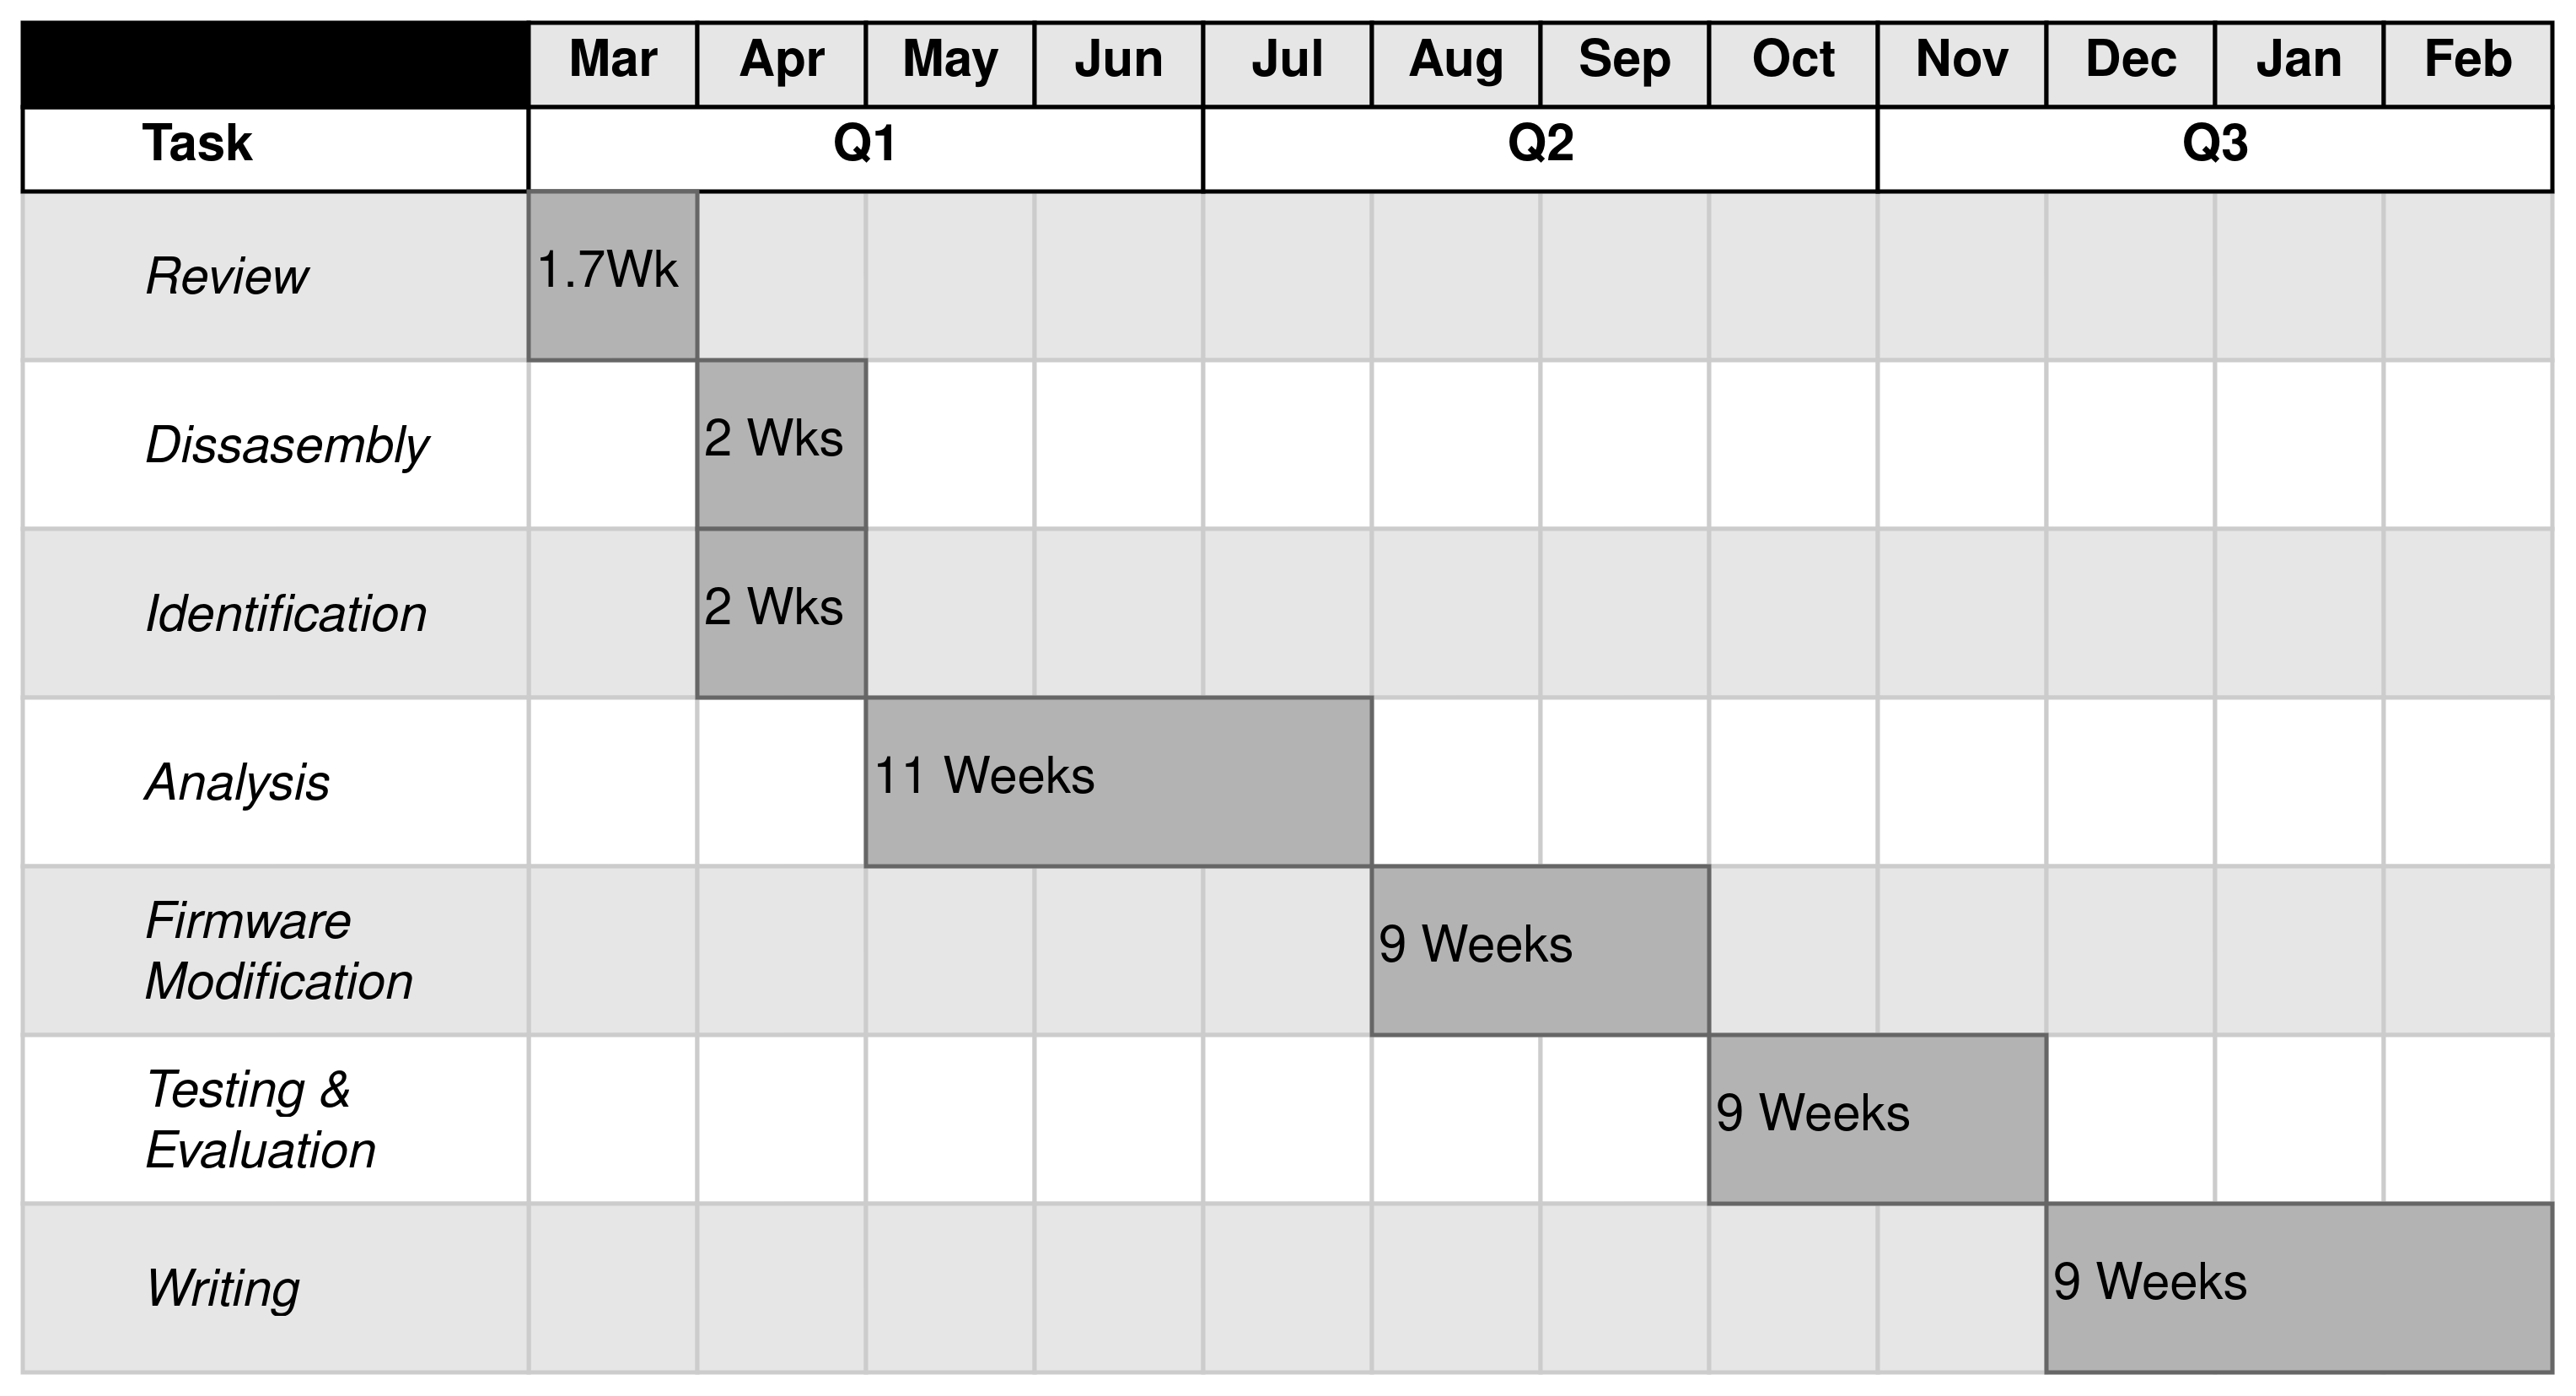
\includegraphics[width=160mm,scale=1]{Figures/timeline_gantt.drawio.png}}
  \caption{Research lifecycle}%
  \label{fig:research_lifecycle}%
\end{figure}

The timeline for the research proposal is divided into seven parts: review, disassembly, identification, analysis, firmware modification, testing, and writing. The dates provided are rough estimates and will vary as the project progresses. Should any of the tasks take longer than initially estimated, time can be taken from the next or the later writing stage of the dissertation.

The initial phase of the dissertation (e.g., review, disassembly, and identification) is shorter than the rest because the information is readily available and easier to gather. The most difficult step is firmware extraction since it would require manually desoldering the flash chip for retrieval, but that can be completed within a day. If the programming adapter for the component is not already available, then the process could take several more days.

The analysis, modification, evaluation, and writing tasks are equally divided between nine weeks each. This is not hard set, and it is possible that the analysis or modification stages will need more time. However, each task was initially estimated with that in mind; if more time is needed, it can be borrowed from the evaluation and writing stage.

% \begin{itemize}
%   \item \textbf{Review}: Review the proposal before beginning the research process to familiarize with the defined methodology, processes, and scope of project.
%   \item \textbf{Surveying}: Gather the necessary technical data and acquire the devices.
%   \item \textbf{Disassembly}: Each device is torn down, components identified, and documented.
%   \item \textbf{Writing}: All data collected, pictures taken, and documents created will be gathered to create a formal report as dictated by the research purpose.
% \end{itemize}

% \begin{table}[h]
%   \centering
%   \begin{tabular}{ |l||c|c|c| }
%     \hline\rowcolor{gray!30}

%     \textbf{Task} & \textbf{Duration} & \textbf{Start Date} & \textbf{End Date} \\
  
%     \hline

%     % creates empty row
%     % &  &  &  \\
%     % \multicolumn{4}{|c|}{} \\

%     \hline\rowcolor{gray!10} 

%     \textbf{Review} & 7 days & 24 Mar 25 & 30 Mar 25 \\

%     Review proposal comments/feedback & 2 days & 24 Mar 25 & 25 Mar 25 \\
%     Amend any changes & 3 days & 26 Mar 25 & 28 Mar 25 \\
%     Prepare work environment & 2 days & 29 Mar 25 & 30 Mar 25 \\

%     \hline
%     \hline\rowcolor{gray!10} 

%     \textbf{Disassembly} & 7 days & 31 Mar 25 & 06 Apr 25 \\

%     Disassemble printer & 2 days & 31 Mar 25 & 01 Apr 25 \\
%     Document interior/exterior of device & 5 days & 02 Apr 25 & 06 Apr 25 \\

%     \hline
%     \hline\rowcolor{gray!10}

%     \textbf{Identification} & 7 days & 07 Apr 25 & 13 Apr 25 \\

%     Identify device components & 3 days & 07 Apr 25 & 09 Apr 25 \\
%     Attempt hardware debug & 1 days & 10 Apr 25 & 10 Apr 25 \\
%     Identify software/hardware protections & 2 days & 11 Apr 25 & 12 Apr 25 \\
%     Document & 1 days & 13 Apr 25 & 13 Apr 25 \\

%     \hline
%     \hline\rowcolor{gray!10}

%     \textbf{Analysis} &  76 days & 14 Apr 25 & 29 Jun 25 \\

%     Capture network/USB traffic & 7 days & 14 Apr 25 & 20 Apr 25 \\
%     Analyze network/USB traffic & 31 days & 21 Apr 25 & 21 May 25 \\
%     Analyze recovered firmware & 31 days & 22 May 25 & 22 Jun 25 \\
%     Document previous tasks & 7 days & 23 Jun 25 & 29 Jun 25 \\

%     \hline
%     \hline\rowcolor{gray!10}

%     \textbf{Firmware Modification} & 62 days & 30 Jun 25 & 31 Aug 25 \\

%     Modify existing firmware & 31 days & 30 Jun 25 & 31 Jul 25 \\
%     Modify third-party firmware & 31 days & 01 Aug 25 & 31 Aug 25 \\

%     \hline
%     \hline\rowcolor{gray!10}

%     \textbf{Testing} & 60 days & 01 Sep 25 & 31 Oct 25 \\

%     Setup testing environment & 7 days & 01 Sep 25 & 07 Sep 25 \\
%     Reflash device w/ modified firmware & 14 days & 08 Sep 25 & 21 Sep 25 \\
%     Test print operations & 7 days & 22 Sep 25 & 28 Sep 25 \\
%     Test HID attacks & 7 days & 29 Sep 25 & 05 Oct 25 \\
%     Make changes and retest & 25 days & 06 Oct 25 & 31 Oct 25 \\

%     \hline
%     \hline\rowcolor{gray!10}

%     \textbf{Extra} & 30 days & 01 Nov 25 & 30 Nov 25 \\
    
%     \hline
%     \hline\rowcolor{gray!10}

%     \textbf{Writing} & 62 days & 01 Dec 25 & 31 Jan 25 \\

%     % \hline
%     % \hline\rowcolor{gray!30}
%     % \textbf{Entire research process} & 42 days & 06 Nov 25 & 18 Dec 25 \\

%     \hline
%   \end{tabular}
%   \caption{Research lifecycle}
%   \label{fig:research_lifecycle}%
% \end{table}


% % Chapter 6
% \section{Conclusion}

% \textbf{Outline}
% $\downarrow$

% \begin{itemize}
%     \item Reiterate the introduction, research questions, and how the results of the research answered those questions.
%     \item Provide supporting statements for future research and highlight areas that were loosely documented/known and would have been solid preliminary research.
%     \item Can these devices be extended? Research questions, yes/no...
% \end{itemize}

% \begin{itemize}
%     \item Summary of physical protections (e.g., too much information silkscreened on PCB)
%     \item List hardware protections (e.g., did manufacturer block debug access, are memory regions locked)
%     \item Discuss software protections (e.g., access to bootloader, identifiable CVEs/CWEs, attributable libraries/functions)
% \end{itemize}

In conclusion, the researcher was able to demonstrate four of the five objectives for the research. We identified baseline of the hardware and operating system used by the serial printer. We identified the specific version of the operating system, any supporting libraries as well as their versions (i.e., RT-Thread RTOS). We were also able to clearly demonstrate that the manufacturers have enabled minimal security protections despite the hardware supporting them; which, is especially worth noting because the operating system itself has minimal protections for isolating memory across processes other than CRC checksums. It is also possible, as demonstrated, to be able to reflash the memory utilizing the MCU hardware debug interfaces.

Due to underestimating the time needed for delivery of the additional devices for the proposed sample population, only one device was assessed. Although the SNBC BTP-S80 is a fairly common serial printer used across financial sectors as well as industrial control, the research would have been better represented with the cross-examination against several other devices. Lastly, another goal of the research was to use the gathered data to support the proposal of future research into a design artifact for implementing BadUSB-like concepts on peripheral serial devices. 

%%% % Evaluations
%%% \chapter*{Self-Evaluation}

%%% Commented out because this is no longer needed (outline only)
%%% \addcontentsline{toc}{chapter}{Self-Evaluation}
\label{chap:evaluation}

Lockwood's three standards ratings:
\begin{itemize}
  \item intellectually original [0 - 5] ... (4): I think the research goals and proposed research are novel in terms of their contributions and application of existing research. It's important to take research, see where it can be applied and then actually prove that it can be. With this project it is more than taking an exactly replicable idea and tossing it at an undocumented piece of hardware. It will require significant research and development time.

  \item technically substantial [0 - 5] ... (3): Again, the ideas are out there and have been used similarly. But they have not been used for this type of device nor type of platform. The exact definitions for how this differentiates from previous works could use some massaging to prevent confusion.

  \item socially constructive [0 - 5] ... (3): Similar to the second standard, finding the exact wording to stress the significance and utility of the work is required. Regardless, these devices are seen everywhere and not just on PoS systems. They can be found on critical infrastructure and industrial control systems or human-machine interfaces where paper reporting is used. Assessment and then creation of a proof-of-concept as future work would, in my eyes, be a novel contribution.
\end{itemize}

\clearpage

% Appendices
%========================================
% \begin{appendices}

\addtocontents{toc}{\protect\renewcommand{\protect\cftchappresnum}{\appendixname\space}}
\addtocontents{toc}{\protect\renewcommand{\protect\cftchapnumwidth}{7em}}

\chapter{This is Appendix A}
\lipsum[1]

\end{appendices}
% \clearpage

% \begin{appendices}

\addtocontents{toc}{\protect\renewcommand{\protect\cftchappresnum}{\appendixname\space}}
\addtocontents{toc}{\protect\renewcommand{\protect\cftchapnumwidth}{7em}}

\chapter{This is Appendix B}
\lipsum[1]

\end{appendices}
% \clearpage

% Reference
%========================================
\addcontentsline{toc}{chapter}{References}
\begin{singlespace}
	\setlength\bibitemsep{\baselineskip}
	\printbibliography[title={References}]
\end{singlespace}
\clearpage

\end{document}